
\documentclass{article}

\usepackage[left=1.8cm,right=1.8cm, top=2cm, bottom = 2cm]{geometry}
\usepackage{amsfonts}

\usepackage{amsmath}
\usepackage{xcolor}

\usepackage{tikz}
\usepackage{subfigure}

\usepackage{pgfplots}

\pgfplotsset{compat=1.10}
\usepgfplotslibrary{fillbetween}
\usetikzlibrary{patterns}



\pagestyle{empty}

\setlength{\tabcolsep}{15pt}


\newcommand{\deriv}[3][]{\frac{\mathrm{d}^{#1}#2}{\mathrm{d}#3^{#1}}}
\newcommand{\diff}{\;\mathrm{d}}

\newcommand{\norm}[1]{\left|\kern-1pt\left|#1\right|\kern-1pt\right|}
\newcommand{\bra}[1]{\left\langle #1 \,\right|}
\newcommand{\ket}[1]{\left|\, #1\right\rangle}
\newcommand{\braket}[2]{\left\langle #1 \mid #2 \right\rangle}




\begin{document}

\title{Convolutions}
\date{}

\maketitle
\thispagestyle{empty}

\Large

\vskip -10mm

\textbf{\underline{Objective: To understand the convolution of two functions and its}}

\textbf{\underline{relationship with multiplication.}}






\vspace{5mm}












\textbf{Warm-up: Cross-Correlation:}

\bigskip


Consider the functions $f(t)=\sin(t)$ and $g(t)=\cos(t)$. These functions are horizontal translations (phase shifts) of each other: $\sin(t)=\cos\left(t-\frac{\pi}{2}\right)$. Let's pretend we don't already know this; we will see how we could find the best amount to translate $\cos(t)$ by to make it similar to $\sin(t)$, using knowledge of the integrals of sine and cosine. This technique will then allow us to study more complicated functions than simple sinusoids.\medskip

The idea is that we will use the inner product of $\sin(t)$ and $\cos(t)$ on $L_2([0,2\pi])$ to compare how similar they are; but we will translate $\cos(t)$ by different amounts, to see how much we need to translate by to make the two functions as similar as possible.

The \textbf{cross-correlation} of $\sin(t)$ and $\cos(t)$ between $0$ and $2\pi$ is
\[\braket{\sin(\tau)}{\cos(\tau+t)}=\int_{0}^{2\pi}\sin(\tau)\cos(\tau+t)\diff \tau.\]

Note that previously we have used an inner product with a factor of $\frac{2}{L}$ in front; this isn't important, so for our current purposes we'll drop this factor, so technically this is a different inner product to the one we've used before, but it differs only by a constant factor, so it's essentially the same. This cross-correlation tells us, for a given $t$, how similar the sine and cosine waves are once the cosine is translated by $t$. See graphs overleaf.\bigskip


\begin{enumerate}
	\item Show that the cross-correlation of sine and cosine is given by
		\[\braket{\sin(\tau)}{\cos(\tau+t)}=-\pi\sin(t).\]
	\item Hence show that the maximum cross-correlation between sine and cosine occurs at $t=-\frac{\pi}{2}$; so $\cos\left(t-\frac{\pi}{2}\right)$ is the most similar a cosine wave can get to a sine wave. In this case, of course, $\cos\left(t-\frac{\pi}{2}\right)$ is actually equal to $\sin(t)$, but we can generalise this to pairs of functions where a simple translation does not turn one exactly into the other.
\end{enumerate}




\clearpage



\begin{center}
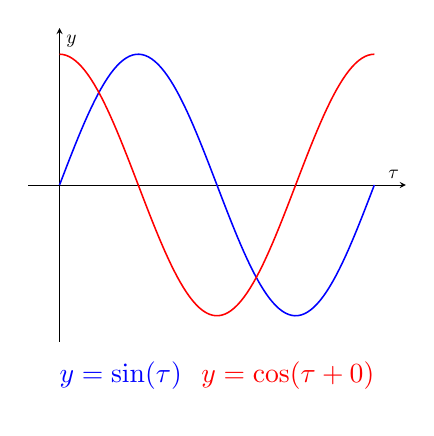
\begin{tikzpicture}[scale=0.7]
	\begin{axis}[axis lines=middle,
		            xlabel=$\tau$,
		            ylabel=$y$,
	           	 enlargelimits,
           		 ytick=\empty,
		            xtick=\empty
           	 ]
		
		\addplot[name path=F,blue,thick,domain={0:6.28},samples=100] {2*sin(x*180/3.14)};

		\addplot[name path=G,red,thick,domain={0:6.28},samples=100] {2*cos((x+0*0.785)*180/3.14)};
	\end{axis}
		\matrix[below] at (current bounding box.south){
			\node[blue,left] {$y=\sin(\tau)$};
			\node[red,right] {$y=\cos(\tau+0)$};\\
		};
\end{tikzpicture}
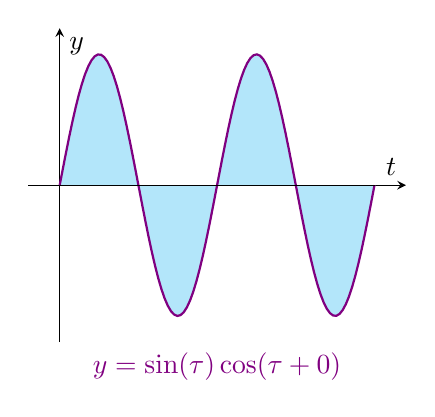
\begin{tikzpicture}[scale=0.7]
	\begin{axis}[axis lines=middle,
		            xlabel=$t$,
		            ylabel=$y$,
	           	 enlargelimits,
           		 ytick=\empty,
		            xtick=\empty
           	 ]
		
		\addplot[name path=F,violet,thick,domain={0:6.28},samples=100] {2*sin(x*180/3.14)*cos((x+0*0.785)*180/3.14)};

		\addplot[name path=G,domain=0:6.28] {0};

		\addplot[cyan!30] fill between [of=F and G];
	\end{axis}
	\node[below,violet] at (current bounding box.south) {$y=\sin(\tau)\cos(\tau+0)$};
\end{tikzpicture}
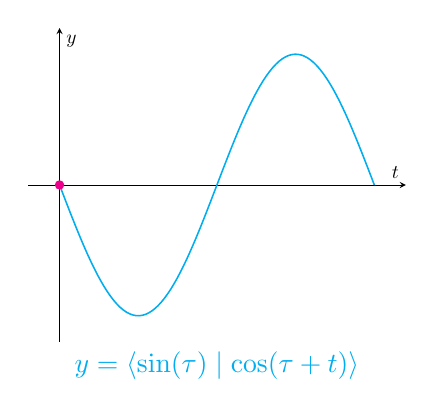
\begin{tikzpicture}[scale=0.7]
	\begin{axis}[axis lines=middle,
		            xlabel=$t$,
		            ylabel=$y$,
	           	 enlargelimits,
           		 ytick=\empty,
		            xtick=\empty
           	 ]
		
		\addplot[name path=F,cyan,thick,domain={0:6.28},samples=100] {-3.14*sin(x*180/3.14)};
		\addplot[magenta,thick,mark=*] coordinates{({0*0.785},{-3.14*sin((0*0.785)*180/3.14))})};
	\end{axis}
	\node[below,cyan] at (current bounding box.south) {$y=\braket{\sin(\tau)}{\cos(\tau+t)}$};
\end{tikzpicture}




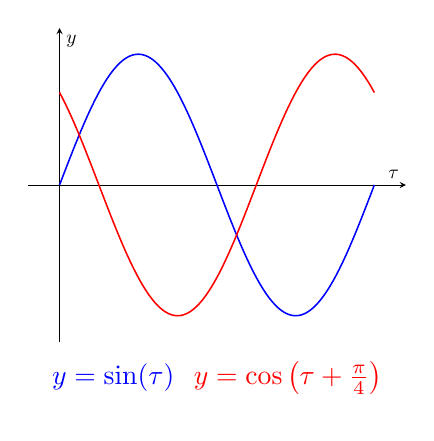
\begin{tikzpicture}[scale=0.7]
	\begin{axis}[axis lines=middle,
		            xlabel=$\tau$,
		            ylabel=$y$,
	           	 enlargelimits,
           		 ytick=\empty,
		            xtick=\empty
           	 ]
		
		\addplot[name path=F,blue,thick,domain={0:6.28},samples=100] {2*sin(x*180/3.14)};

		\addplot[name path=G,red,thick,domain={0:6.28},samples=100] {2*cos((x+1*0.785)*180/3.14)};
	\end{axis}
		\matrix[below] at (current bounding box.south){
			\node[blue,left] {$y=\sin(\tau)$};
			\node[red,right] {$y=\cos\left(\tau+\frac{\pi}{4}\right)$};\\
		};
\end{tikzpicture}
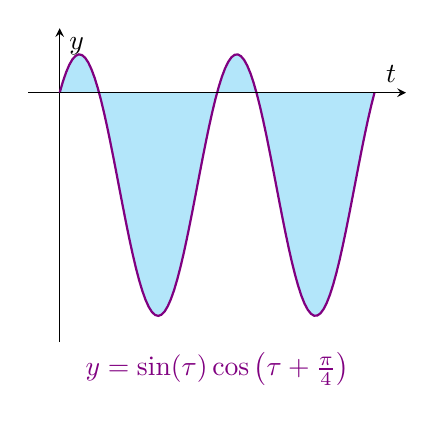
\begin{tikzpicture}[scale=0.7]
	\begin{axis}[axis lines=middle,
		            xlabel=$t$,
		            ylabel=$y$,
	           	 enlargelimits,
           		 ytick=\empty,
		            xtick=\empty
           	 ]
		
		\addplot[name path=F,violet,thick,domain={0:6.28},samples=100] {2*sin(x*180/3.14)*cos((x+1*0.785)*180/3.14)};

		\addplot[name path=G,domain=0:6.28] {0};

		\addplot[cyan!30] fill between [of=F and G];
	\end{axis}
	\node[below,violet] at (current bounding box.south) {$y=\sin(\tau)\cos\left(\tau+\frac{\pi}{4}\right)$};
\end{tikzpicture}
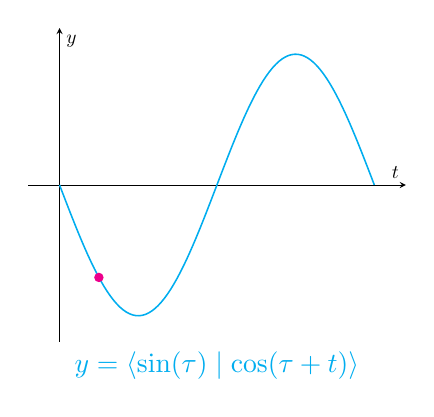
\begin{tikzpicture}[scale=0.7]
	\begin{axis}[axis lines=middle,
		            xlabel=$t$,
		            ylabel=$y$,
	           	 enlargelimits,
           		 ytick=\empty,
		            xtick=\empty
           	 ]
		
		\addplot[name path=F,cyan,thick,domain={0:6.28},samples=100] {-3.14*sin(x*180/3.14)};
		\addplot[magenta,thick,mark=*] coordinates{({1*0.785},{-3.14*sin((1*0.785)*180/3.14))})};
	\end{axis}
	\node[below,cyan] at (current bounding box.south) {$y=\braket{\sin(\tau)}{\cos(\tau+t)}$};
\end{tikzpicture}




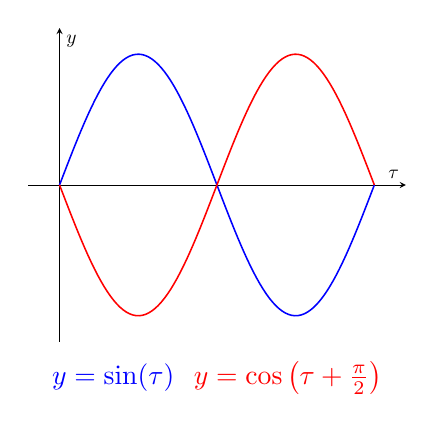
\begin{tikzpicture}[scale=0.7]
	\begin{axis}[axis lines=middle,
		            xlabel=$\tau$,
		            ylabel=$y$,
	           	 enlargelimits,
           		 ytick=\empty,
		            xtick=\empty
           	 ]
		
		\addplot[name path=F,blue,thick,domain={0:6.28},samples=100] {2*sin(x*180/3.14)};

		\addplot[name path=G,red,thick,domain={0:6.28},samples=100] {2*cos((x+2*0.785)*180/3.14)};
	\end{axis}
		\matrix[below] at (current bounding box.south){
			\node[blue,left] {$y=\sin(\tau)$};
			\node[red,right] {$y=\cos\left(\tau+\frac{\pi}{2}\right)$};\\
		};
\end{tikzpicture}
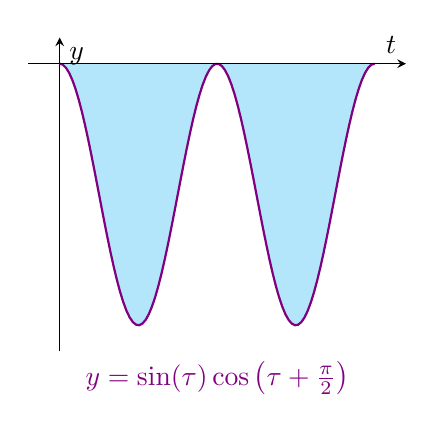
\begin{tikzpicture}[scale=0.7]
	\begin{axis}[axis lines=middle,
		            xlabel=$t$,
		            ylabel=$y$,
	           	 enlargelimits,
           		 ytick=\empty,
		            xtick=\empty
           	 ]
		
		\addplot[name path=F,violet,thick,domain={0:6.28},samples=100] {2*sin(x*180/3.14)*cos((x+2*0.785)*180/3.14)};

		\addplot[name path=G,domain=0:6.28] {0};

		\addplot[cyan!30] fill between [of=F and G];
	\end{axis}
	\node[below,violet] at (current bounding box.south) {$y=\sin(\tau)\cos\left(\tau+\frac{\pi}{2}\right)$};
\end{tikzpicture}
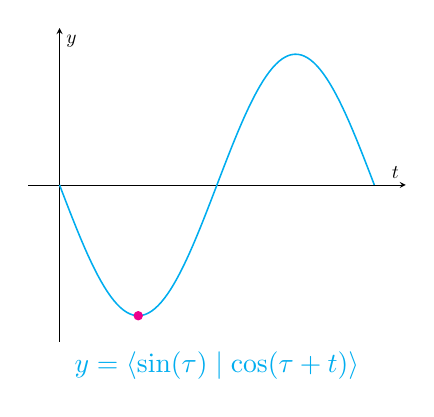
\begin{tikzpicture}[scale=0.7]
	\begin{axis}[axis lines=middle,
		            xlabel=$t$,
		            ylabel=$y$,
	           	 enlargelimits,
           		 ytick=\empty,
		            xtick=\empty
           	 ]
		
		\addplot[name path=F,cyan,thick,domain={0:6.28},samples=100] {-3.14*sin(x*180/3.14)};
		\addplot[magenta,thick,mark=*] coordinates{({2*0.785},{-3.14*sin((2*0.785)*180/3.14))})};
	\end{axis}
	\node[below,cyan] at (current bounding box.south) {$y=\braket{\sin(\tau)}{\cos(\tau+t)}$};
\end{tikzpicture}




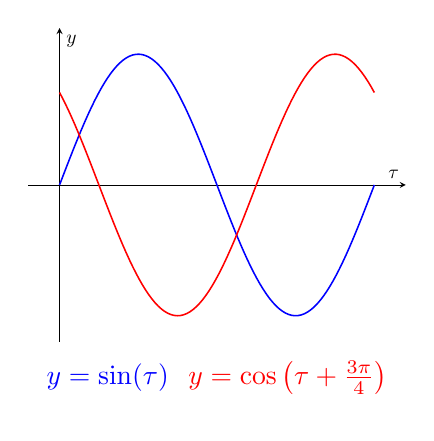
\begin{tikzpicture}[scale=0.7]
	\begin{axis}[axis lines=middle,
		            xlabel=$\tau$,
		            ylabel=$y$,
	           	 enlargelimits,
           		 ytick=\empty,
		            xtick=\empty
           	 ]
		
		\addplot[name path=F,blue,thick,domain={0:6.28},samples=100] {3*sin(x*180/3.14)};

		\addplot[name path=G,red,thick,domain={0:6.28},samples=100] {3*cos((x+1*0.785)*180/3.14)};
	\end{axis}
		\matrix[below] at (current bounding box.south){
			\node[blue,left] {$y=\sin(\tau)$};
			\node[red,right] {$y=\cos\left(\tau+\frac{3\pi}{4}\right)$};\\
		};
\end{tikzpicture}
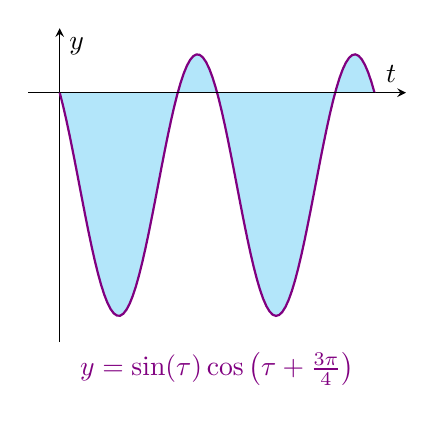
\begin{tikzpicture}[scale=0.7]
	\begin{axis}[axis lines=middle,
		            xlabel=$t$,
		            ylabel=$y$,
	           	 enlargelimits,
           		 ytick=\empty,
		            xtick=\empty
           	 ]
		
		\addplot[name path=F,violet,thick,domain={0:6.28},samples=100] {2*sin(x*180/3.14)*cos((x+3*0.785)*180/3.14)};

		\addplot[name path=G,domain=0:6.28] {0};

		\addplot[cyan!30] fill between [of=F and G];
	\end{axis}
	\node[below,violet] at (current bounding box.south) {$y=\sin(\tau)\cos\left(\tau+\frac{3\pi}{4}\right)$};
\end{tikzpicture}
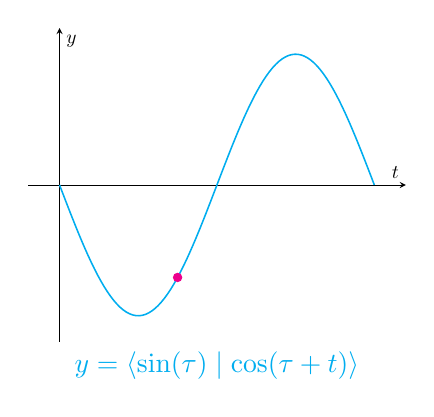
\begin{tikzpicture}[scale=0.7]
	\begin{axis}[axis lines=middle,
		            xlabel=$t$,
		            ylabel=$y$,
	           	 enlargelimits,
           		 ytick=\empty,
		            xtick=\empty
           	 ]
		
		\addplot[name path=F,cyan,thick,domain={0:6.28},samples=100] {-3.14*sin(x*180/3.14)};
		\addplot[magenta,thick,mark=*] coordinates{({3*0.785},{-3.14*sin((3*0.785)*180/3.14))})};
	\end{axis}
	\node[below,cyan] at (current bounding box.south) {$y=\braket{\sin(\tau)}{\cos(\tau+t)}$};
\end{tikzpicture}




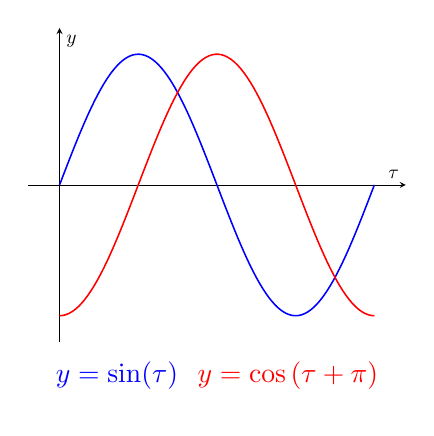
\begin{tikzpicture}[scale=0.7]
	\begin{axis}[axis lines=middle,
		            xlabel=$\tau$,
		            ylabel=$y$,
	           	 enlargelimits,
           		 ytick=\empty,
		            xtick=\empty
           	 ]
		
		\addplot[name path=F,blue,thick,domain={0:6.28},samples=100] {2*sin(x*180/3.14)};

		\addplot[name path=G,red,thick,domain={0:6.28},samples=100] {2*cos((x+4*0.785)*180/3.14)};
	\end{axis}
		\matrix[below] at (current bounding box.south){
			\node[blue,left] {$y=\sin(\tau)$};
			\node[red,right] {$y=\cos\left(\tau+\pi\right)$};\\
		};
\end{tikzpicture}
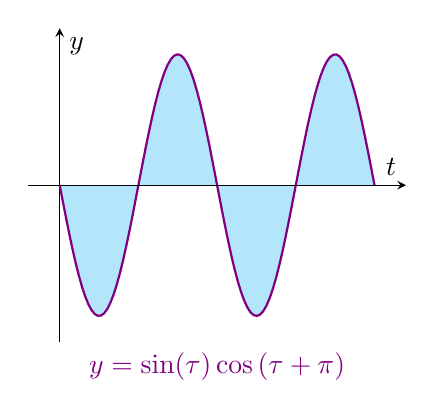
\begin{tikzpicture}[scale=0.7]
	\begin{axis}[axis lines=middle,
		            xlabel=$t$,
		            ylabel=$y$,
	           	 enlargelimits,
           		 ytick=\empty,
		            xtick=\empty
           	 ]
		
		\addplot[name path=F,violet,thick,domain={0:6.28},samples=100] {2*sin(x*180/3.14)*cos((x+4*0.785)*180/3.14)};

		\addplot[name path=G,domain=0:6.28] {0};

		\addplot[cyan!30] fill between [of=F and G];
	\end{axis}
	\node[below,violet] at (current bounding box.south) {$y=\sin(\tau)\cos\left(\tau+\pi\right)$};
\end{tikzpicture}
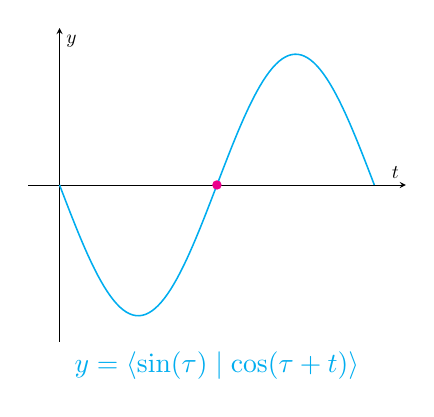
\begin{tikzpicture}[scale=0.7]
	\begin{axis}[axis lines=middle,
		            xlabel=$t$,
		            ylabel=$y$,
	           	 enlargelimits,
           		 ytick=\empty,
		            xtick=\empty
           	 ]
		
		\addplot[name path=F,cyan,thick,domain={0:6.28},samples=100] {-3.14*sin(x*180/3.14)};
		\addplot[magenta,thick,mark=*] coordinates{({4*0.785},{-3.14*sin((4*0.785)*180/3.14))})};
	\end{axis}
	\node[below,cyan] at (current bounding box.south) {$y=\braket{\sin(\tau)}{\cos(\tau+t)}$};
\end{tikzpicture}




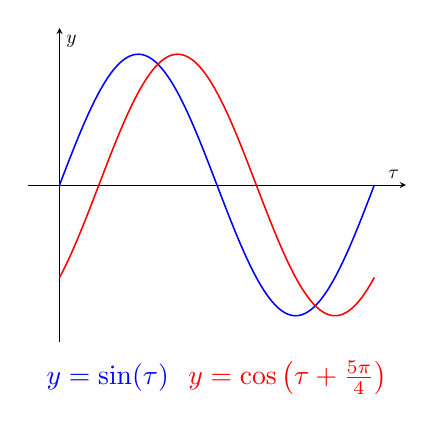
\begin{tikzpicture}[scale=0.7]
	\begin{axis}[axis lines=middle,
		            xlabel=$\tau$,
		            ylabel=$y$,
	           	 enlargelimits,
           		 ytick=\empty,
		            xtick=\empty
           	 ]
		
		\addplot[name path=F,blue,thick,domain={0:6.28},samples=100] {2*sin(x*180/3.14)};

		\addplot[name path=G,red,thick,domain={0:6.28},samples=100] {2*cos((x+5*0.785)*180/3.14)};
	\end{axis}
		\matrix[below] at (current bounding box.south){
			\node[blue,left] {$y=\sin(\tau)$};
			\node[red,right] {$y=\cos\left(\tau+\frac{5\pi}{4}\right)$};\\
		};
\end{tikzpicture}
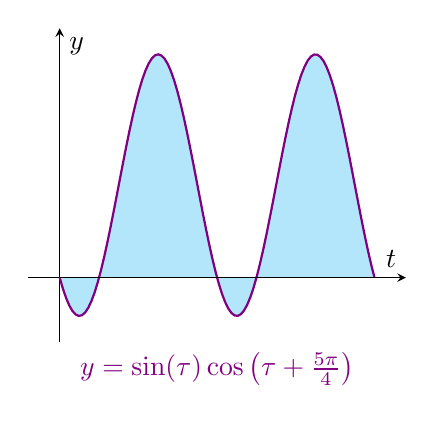
\begin{tikzpicture}[scale=0.7]
	\begin{axis}[axis lines=middle,
		            xlabel=$t$,
		            ylabel=$y$,
	           	 enlargelimits,
           		 ytick=\empty,
		            xtick=\empty
           	 ]
		
		\addplot[name path=F,violet,thick,domain={0:6.28},samples=100] {2*sin(x*180/3.14)*cos((x+5*0.785)*180/3.14)};

		\addplot[name path=G,domain=0:6.28] {0};

		\addplot[cyan!30] fill between [of=F and G];
	\end{axis}
	\node[below,violet] at (current bounding box.south) {$y=\sin(\tau)\cos\left(\tau+\frac{5\pi}{4}\right)$};
\end{tikzpicture}
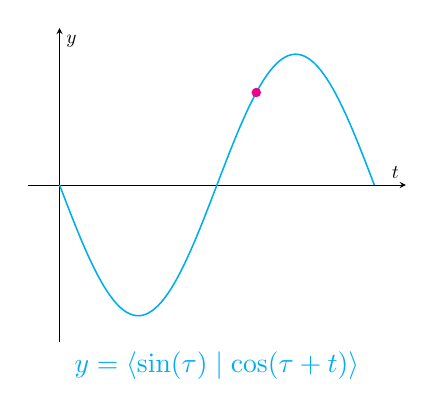
\begin{tikzpicture}[scale=0.7]
	\begin{axis}[axis lines=middle,
		            xlabel=$t$,
		            ylabel=$y$,
	           	 enlargelimits,
           		 ytick=\empty,
		            xtick=\empty
           	 ]
		
		\addplot[name path=F,cyan,thick,domain={0:6.28},samples=100] {-3.14*sin(x*180/3.14)};
		\addplot[magenta,thick,mark=*] coordinates{({5*0.785},{-3.14*sin((5*0.785)*180/3.14))})};
	\end{axis}
	\node[below,cyan] at (current bounding box.south) {$y=\braket{\sin(\tau)}{\cos(\tau+t)}$};
\end{tikzpicture}




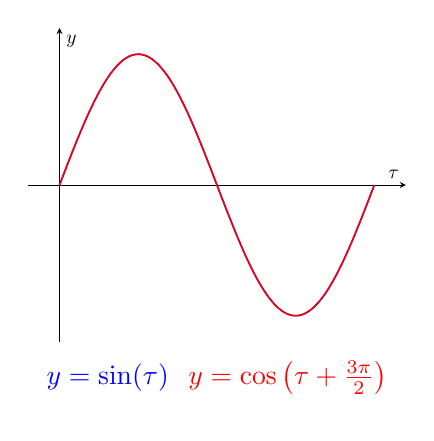
\begin{tikzpicture}[scale=0.7]
	\begin{axis}[axis lines=middle,
		            xlabel=$\tau$,
		            ylabel=$y$,
	           	 enlargelimits,
           		 ytick=\empty,
		            xtick=\empty
           	 ]
		
		\addplot[name path=F,blue,thick,domain={0:6.28},samples=100] {2*sin(x*180/3.14)};

		\addplot[name path=G,red,thick,domain={0:6.28},samples=100] {2*cos((x+6*0.785)*180/3.14)};
	\end{axis}
		\matrix[below] at (current bounding box.south){
			\node[blue,left] {$y=\sin(\tau)$};
			\node[red,right] {$y=\cos\left(\tau+\frac{3\pi}{2}\right)$};\\
		};
\end{tikzpicture}
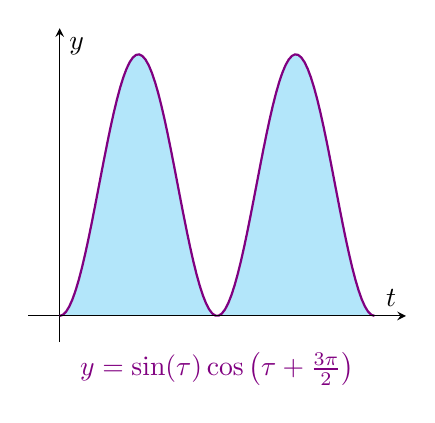
\begin{tikzpicture}[scale=0.7]
	\begin{axis}[axis lines=middle,
		            xlabel=$t$,
		            ylabel=$y$,
	           	 enlargelimits,
           		 ytick=\empty,
		            xtick=\empty
           	 ]
		
		\addplot[name path=F,violet,thick,domain={0:6.28},samples=100] {2*sin(x*180/3.14)*cos((x+6*0.785)*180/3.14)};

		\addplot[name path=G,domain=0:6.28] {0};

		\addplot[cyan!30] fill between [of=F and G];
	\end{axis}
	\node[below,violet] at (current bounding box.south) {$y=\sin(\tau)\cos\left(\tau+\frac{3\pi}{2}\right)$};
\end{tikzpicture}
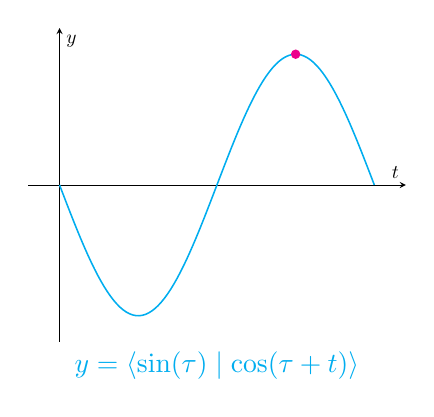
\begin{tikzpicture}[scale=0.7]
	\begin{axis}[axis lines=middle,
		            xlabel=$t$,
		            ylabel=$y$,
	           	 enlargelimits,
           		 ytick=\empty,
		            xtick=\empty
           	 ]
		
		\addplot[name path=F,cyan,thick,domain={0:6.28},samples=100] {-3.14*sin(x*180/3.14)};
		\addplot[magenta,thick,mark=*] coordinates{({6*0.785},{-3.14*sin((6*0.785)*180/3.14))})};
	\end{axis}
	\node[below,cyan] at (current bounding box.south) {$y=\braket{\sin(\tau)}{\cos(\tau+t)}$};
\end{tikzpicture}




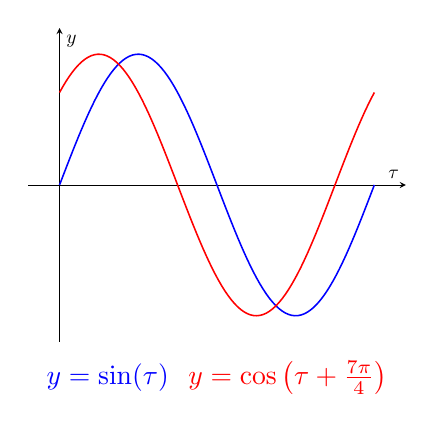
\begin{tikzpicture}[scale=0.7]
	\begin{axis}[axis lines=middle,
		            xlabel=$\tau$,
		            ylabel=$y$,
	           	 enlargelimits,
           		 ytick=\empty,
		            xtick=\empty
           	 ]
		
		\addplot[name path=F,blue,thick,domain={0:6.28},samples=100] {2*sin(x*180/3.14)};

		\addplot[name path=G,red,thick,domain={0:6.28},samples=100] {2*cos((x+7*0.785)*180/3.14)};
	\end{axis}
		\matrix[below] at (current bounding box.south){
			\node[blue,left] {$y=\sin(\tau)$};
			\node[red,right] {$y=\cos\left(\tau+\frac{7\pi}{4}\right)$};\\
		};
\end{tikzpicture}
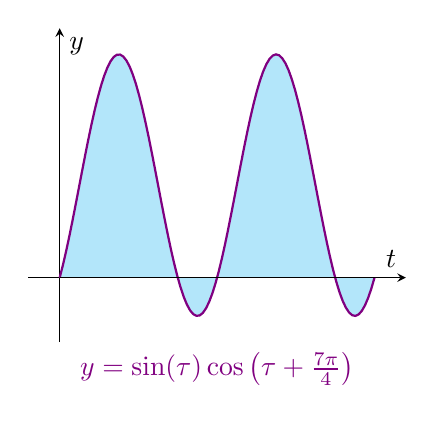
\begin{tikzpicture}[scale=0.7]
	\begin{axis}[axis lines=middle,
		            xlabel=$t$,
		            ylabel=$y$,
	           	 enlargelimits,
           		 ytick=\empty,
		            xtick=\empty
           	 ]
		
		\addplot[name path=F,violet,thick,domain={0:6.28},samples=100] {2*sin(x*180/3.14)*cos((x+7*0.785)*180/3.14)};

		\addplot[name path=G,domain=0:6.28] {0};

		\addplot[cyan!30] fill between [of=F and G];
	\end{axis}
	\node[below,violet] at (current bounding box.south) {$y=\sin(\tau)\cos\left(\tau+\frac{7\pi}{4}\right)$};
\end{tikzpicture}
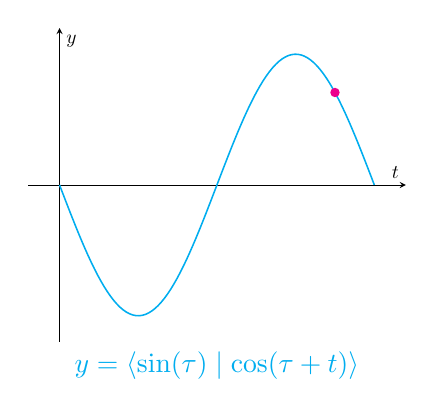
\begin{tikzpicture}[scale=0.7]
	\begin{axis}[axis lines=middle,
		            xlabel=$t$,
		            ylabel=$y$,
	           	 enlargelimits,
           		 ytick=\empty,
		            xtick=\empty
           	 ]
		
		\addplot[name path=F,cyan,thick,domain={0:6.28},samples=100] {-3.14*sin(x*180/3.14)};
		\addplot[magenta,thick,mark=*] coordinates{({7*0.785},{-3.14*sin((7*0.785)*180/3.14))})};
	\end{axis}
	\node[below,cyan] at (current bounding box.south) {$y=\braket{\sin(\tau)}{\cos(\tau+t)}$};
\end{tikzpicture}
\end{center}








\clearpage












\textbf{Theory: Convolution:}\bigskip


The cross-correlation of two functions $f$ and $g$ tells you, for each $t$, broadly how similar $f(\tau)$ and $g(\tau+t)$ are. There is a similar notion, called the \textbf{convolution} of $f$ and $g$, denoted $(f\ast g)(t)$, which tells you for each $t$ how similar $f(\tau)$ and $g(t-\tau)$ are; so the convolution of $f(t)$ with $g(t)$ is simply the cross-correlation of $f(t)$ with $g(-t)$.

Above, we considered the cross-correlation of periodic functions, sine and cosine, so it made sense to integrate over one period. In general, we will integrate over the whole real line. So
\[(f\ast g)(t)=\int_{-\infty}^\infty f(\tau)g(t-\tau)\diff \tau.\]
Of course, this integral might not converge; if $f$ and $g$ are $L_2$ functions, it will (by essentially the same argument as for the convergence of the inner product). If $f$ and $g$ are not square-integrable, then by broadening our notion of functions to include functionals like the Dirac delta, we can often still convolve $f$ and $g$, just as we can take Fourier transforms of non-square-integrable functions.\bigskip



Suppose we have two time-domain functions, $f(t)$ and $g(t)$, whose Fourier transforms $\hat{f}(\omega)$ and $\hat{g}(\omega)$ are known. Can we use this to compute the Fourier transform of the convolution, $f\ast g$? We have:
\begin{align*}
	\widehat{f\ast g}(\omega) &=\int_{-\infty}^\infty (f\ast g)(t)e^{-i\omega t}\diff t\\
	&=\int_{-\infty}^\infty\int_{-\infty}^\infty f(\tau)g(t-\tau)\diff \tau\,e^{-i\omega t}\diff t\\
	&=\iint_{\mathbb{R}^2} f(\tau)g(t-\tau)e^{-i\omega t}\diff \tau\diff t.
\end{align*}

Now we substitute $\sigma=t-\tau$ in the outer integral (so $\diff \sigma =\diff t$):
\begin{align*}
	\widehat{f\ast g}(\omega)&= \iint_{\mathbb{R}^2} f(\tau)g(\sigma)e^{-i\omega (\tau+\sigma)}\diff \tau\diff\sigma\\
	&=\iint_{\mathbb{R}^2}f(\tau)e^{-i\omega \tau}g(\sigma)e^{-i\omega \sigma}\diff \tau\diff \sigma\\
	&=\int_{-\infty}^\infty g(\sigma) e^{-i\omega \sigma}\int_{-\infty}^\infty f(\tau)e^{-i\omega \tau}\diff \tau \diff\sigma\\
	&=\int_{-\infty}^\infty f(\tau)e^{-i\omega \tau}\diff \tau \int_{-\infty}^\infty g(\sigma)e^{-i\omega \sigma}\diff\sigma\\
	&=\hat{f}(\omega)\hat{g}(\omega).
\end{align*}


\clearpage


\textbf{Theory: Convolution (cont.):}\bigskip


So for time-domain functions $f$ and $g$, the Fourier transform of the convolution is the product of the individual Fourier transforms:
\[\widehat{f\ast g}=\hat{f}\hat{g}.\]
We usually express this by saying that convolution in the time domain corresponds to multiplication in the frequency domain.

The converse is also true (up to a constant): multiplication in the time domain corresponds to convolution in the frequency domain:
\[\widehat{fg}=\frac{1}{2\pi}\hat{f}\ast \hat{g}.\]

Depending on the conventions used in defining the forward and inverse transforms, the factor of $\frac{1}{2\pi}$ can be split as a factor of $\frac{1}{\sqrt{2\pi}}$ on both of the two equations above, or can be absent entirely, if ordinary instead of angular frequency is used. The proof of the converse formula is essentially the same as the proof of the forward formula; take the inverse transform of $\hat{f}\ast\hat{g}$ and apply the same manipulations as we did on the previous page.\bigskip


The direct use of this relationship between multiplication and convolution is that if we know the Fourier transforms of functions $f$ and $g$, and wish to find the transform of $fg$, it might be easier to convolve the transforms of $f$ and $g$ than to directly take the transform of $fg$.

Moreover, convolution itself has many applications; for instance, many filtering processes in electronics, acoustics, and optics, amount to convolving a signal with some noise or lens function. In probability, if $X$ and $Y$ are random variables, the probability distribution of $X+Y$ is found by convolving the distributions of $X$ and of $Y$. The Fourier transform allows us to convert convolution problems such as this into multiplication problems; because of Fast Fourier Transform algorithms, it can be computationally quicker to transform two functions, multiply them, then take the inverse transform than it is to convolve them directly.\bigskip


Another use of the Convolution Theorem is that it allows us to prove properties of convolution by relating them to properties of multiplication. For instance, to prove that $f\ast g=g\ast f$, we could work from the definition by the integral, but it's easier just to take the Fourier transform, note that $\hat{f}\hat{g}=\hat{g}\hat{f}$, then take the inverse transform.






\clearpage



\textbf{Practice:}\bigskip

For the following questions, we will use the angular frequency Fourier transform:
\begin{align*}
	\hat{f}(\omega)&=\int_{-\infty}^\infty f(t)e^{-i\omega t}\diff t\\
	f(t)&=\frac{1}{2\pi}\int_{-\infty}^\infty \hat{f}(\omega)e^{i\omega t}\diff t.
\end{align*}

You may assume the following transforms, which we have shown on previous sheets (where $H(t)$ is the Heaviside step function):

\begin{center}
\begin{tabular}{c|c|c}
	$f(t)$ & $\hat{f}(\omega)$ & Conditions\\ \hline
	$H(t)e^{-\alpha t}$ & $\frac{1}{\alpha+i\omega}$ & $\alpha>0$\\ \hline
	$e^{i\alpha t}$ & $\delta(\omega-\alpha)$ & $\alpha\in\mathbb{R}$
\end{tabular}
\end{center}

\begin{enumerate}
	\item Let $\phi(\omega)$ be a frequency-domain function and $\psi(\omega)=\delta(\omega-\alpha)$, where $\delta$ is the Dirac delta.
		\begin{enumerate}
			\item Show that
				\[(\phi \ast \psi)(\omega)=\phi(\omega+\alpha).\]
			\item Hence show that for any time-domain function $f(t)$,
				\[\widehat{f(t)e^{i\alpha t}}(\omega) = \hat{f}(\omega+\alpha).\]
				This is referred to as ``shift in frequency domain.'' Interchanging the roles of the time and frequency domains, we can also show that
				\[\widehat{f(t-\alpha)}=\hat{f}(\omega)e^{-i\alpha\omega}.\]
				This is the formula for ``shift in time domain.''
		\end{enumerate}
	\item Let $f(t)=H(t)e^{-\alpha t}\cos(\beta t)$, for positive real constants $\alpha$ and $\beta$. Show that the Fourier transform of $f$ is
		\[\frac{1}{2(\alpha+i(\omega-\beta))}+\frac{1}{2(\alpha+i(\omega+\beta))}.\]
		Hint: write $\cos(\beta t)$ in terms of complex exponentials, and use question 1(a) for convolution of a function with a Dirac delta.
\end{enumerate}


















\clearpage




{\bf Key Points to Remember:}

\vspace{5mm}

\begin{enumerate}
	\item The \textbf{convolution} of two functions $f$ and $g$ is the function $f\ast g$ defined by
		\[(f\ast g)(t)=\int_{-\infty}^\infty f(\tau)g(t-\tau)\diff \tau.\]
		It gives a measure, for each $t$, of how much $f(\tau)$ and $g(-\tau)$ are similar (in terms of having the same sign) when $g(-\tau)$ is translated by $t$.
	\item The \textbf{convolution theorem} states that convolution and multiplication are dual under the Fourier transform:
		\begin{align*}
			\widehat{f\ast g}&=\hat{f}\hat{g}\\
			\widehat{fg}&=\hat{f}\ast\hat{g}.
		\end{align*}
	\item Convolution with a Dirac delta is translation:
		\[f(t)\ast \delta(t-\alpha) = f(t+\alpha)\]
		for any function $f$.
	\item Using the convolution theorem and the fact that $\delta(\omega-\alpha)$ is the Fourier transform of $e^{i\alpha t}$, we obtain the formulae for time-shift and frequency-shift:
		\begin{align*}
			\widehat{f(t+\alpha)}&= \hat{f}(\omega)e^{i\alpha \omega}\\
			\widehat{f(t)e^{i\alpha t}}(\omega)&=\hat{f}(\omega+\alpha).
		\end{align*}
\end{enumerate}









\end{document}